\chapter{Background}\label{C:back}

\section{Related work}
Much related work has been done in two major areas. Data mining focused techniques with visualisations used to explore the results of data mining, and visualisation driven techniques. Most visualisation driven techniques still contain significant datamining tools. Relatively little work has been done directly on access or system log visualisation, with research preferring to focus on network intrusion detetection logs. For the purposes of this section Intrusion Detection Systems(IDS) are treated as datamining systems. For anomaly based IDS this is straightforward, as they use traditional machine learning and datamining techniques to create classification systems for events. In rule based IDS, this is not so clear, as they apply pre-created rules. However, these rules are often created using data-mining techniques and serve to offer the same black box classification system as other data-mining software. I will be considering how each system discussed below meets the goals set out in Chapter \ref{C:intro}.

\subsection{Data Mining with Visualisation}

LogView \cite{4641277} is a visualisation tool designed to support undertstanding of information extracted through data-mining techniques applied to systems logs. The visualisation component uses treemaps to show clusters of events in a space efficient manner, with leaf nodes representing events, and branches showing clusters the events belong to. All leaf nodes are coloured in green, with shade darkening in 4 steps, representing  statuses OK, WARN, FAIL, OUTLIER in order.  The tool produced allows filtering based on time, and search terms. Time filtering shows only events occuring on the specified day in the map. Nodes matching search terms are highlighted red. Detailed information about a given event is available via mouseover. The simple filtering and interaction methods, coupled with very similar shades for clusters leaves the system very vulnerable to producing information overload in users. The overload potential grows rapidly as the logs grow, as there is very little information hiding present in this tool. 

\begin{figure}[tbh]
\fbox{\parbox[b]{.99\linewidth}{
\vskip 0.5cm
\centering 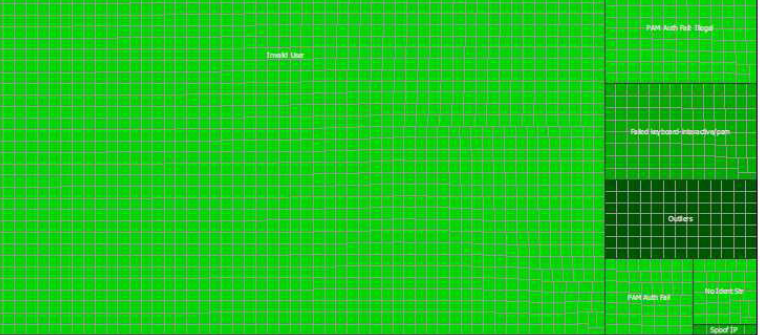
\includegraphics[scale=0.75]{tree.png}
\vskip 0.5cm}}
\caption{\protect\label{tree} LogView treemap of SSHD logs \cite{4641277}. Shades of gree indicate severity of event.}
\end{figure}

A heirarchical system for visualising IDS logs \cite{itoh2006hierarchical} shows an interesting approach to the issue of context for IDS reports. Intrusion detection system messages are lacking in the context needed to support an evaluation of the priority and accuracy of the report. This tool shows the entire network under surveillance using a rectangle packing algorithm to group machines by subnets, the number of incidents sent and recieved from a given machine are displayed as a coloured bar rising out of the plane. This quickly leads to navigability and readability problems as the number of incidents reported grows. Simple filtering tools are available to limit by severity, time, IP and signature ID.
This system is highly reliant on an IDS system with both a low false positive, and false negative rate, as almost all information about the actual events is hidden, and no easy method to drill down to detailed information is provided.

A system log data mining approach is presented by W. Xu et al. \cite{Xu:2009:DLS:1629575.1629587}. This approach uses data mining and machine learning techniques heavily. Log syntax is automatically recovered through source code analysis, allowing the system to be applied to any source available software. Once log synatx is extracted, logs are parsed and machine learning algorithms used to perform feature extraction. Once the features were extracted the principle component analysis anomaly detection algorithm were applied to this data, to find interesting patterns in log messages. This approach identified many issues in the tested software, but was forced to be extended from a pure data-mining approach as users found the black box nature of data-mining algorithms caused difficulty in understanding why the results were as they are. To assist with this, a very simple decision tree visualisation was added, shown in Figure \ref{decision}. This visualisation was created with the intention of showing the logic used by the data-mining systems to give context for decisions. As the processing required for feature extraction and anomaly detection is highly parallel this approach readily scales to millions of entries, and shows very strong performance in detecting anomalous patterns in logs. However, from a security standpoint decision trees alone do not give sufficient context to easily determine if an anomaly represents an intrusion. This depends on much data not included in the raw logs.

\begin{figure}[tbh]
\fbox{\parbox[b]{.99\linewidth}{
\vskip 0.5cm
\centering 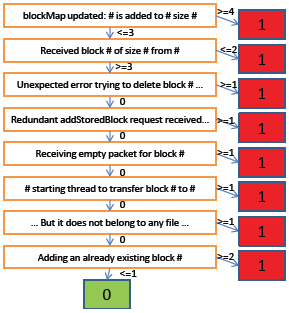
\includegraphics[scale=1]{decisions.png}
\vskip 0.5cm}}
\caption{\protect\label{decision} Decision tree diagram \cite{Xu:2009:DLS:1629575.1629587}. Red 1's indicate anomalies, Green 0 indicates normal. labels on the edges show count thresholds for decisions.}
\end{figure}

\subsection{Visualisation Focused}

Picvis \cite{tricaud2008picviz} is a tool created to generate parallel co-ordinate plots of log data. Picviz offers tools to automate data extraction from several common log formats for use with their plot description language (pcl). This language allows a great deal of control over what variables are shown on a plot. Parallel co-ordinate plots can show strong clustering extremely well. However there are issues of scalability, as clusters and patterns can easily be hidden in background noise unless axes are well chosen. See Figure \ref{parallel}. Filtering tools are available to help address this limitation, but still require significant knowlege of the data structure and content. This tool would be excellent for confirmatory analyses however. 

\begin{figure}[tbh]
\fbox{\parbox[b]{.99\linewidth}{
\vskip 0.5cm
\centering 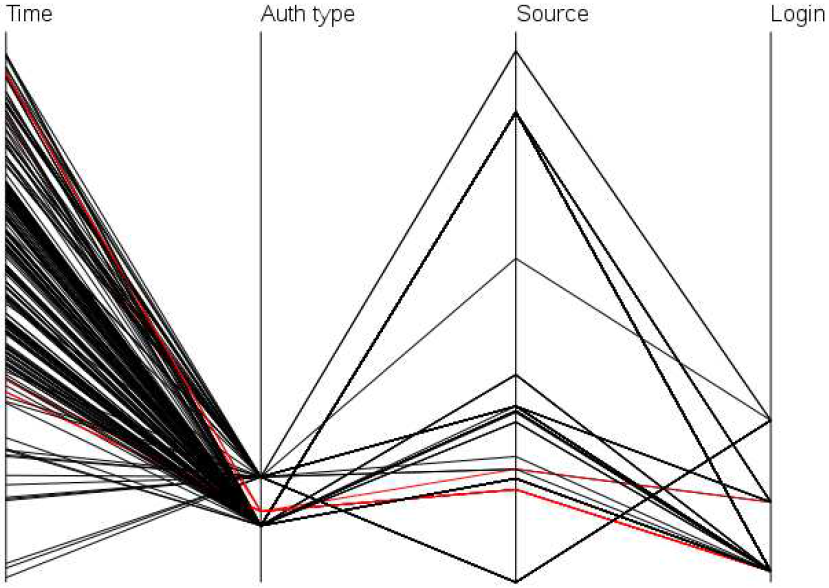
\includegraphics[scale=0.70]{parallel.png}
\vskip 0.5cm}}
\caption{\protect\label{parallel} Picviz parallel plots visualisation \cite{tricaud2008picviz} showing SSH logs.}
\end{figure}

Spiralview \cite{bertini2007spiralview} is a layout technique for timeseries data. Data is laid out in a spiral as shown in Figure \ref{spiral}. This technique has been used both for dynamic data streams \cite{chin2009visual} and analysis of static logs \cite{bertini2007spiralview}. In both applications strong promise is shown intially, as the spiral layout is intuitively expected to effectively reveal repeating patterns in time series data, such as intrusion detection system reports and access logs. However, the paper presenting the spiral technique for use in analysis of static logs does not attempt to evaluate the effectiveness with rigour \cite{bertini2007spiralview}. A rigorous evaluation of the spiral technique was performed in the paper proposing its use for dynamic datastreams \cite{chin2009visual}, However there are severe flaws in the presentation of this evaluation, as the table of results directly contradicts the text. 

\begin{figure}[tbh]
\fbox{\parbox[b]{.99\linewidth}{
\vskip 0.5cm
\centering 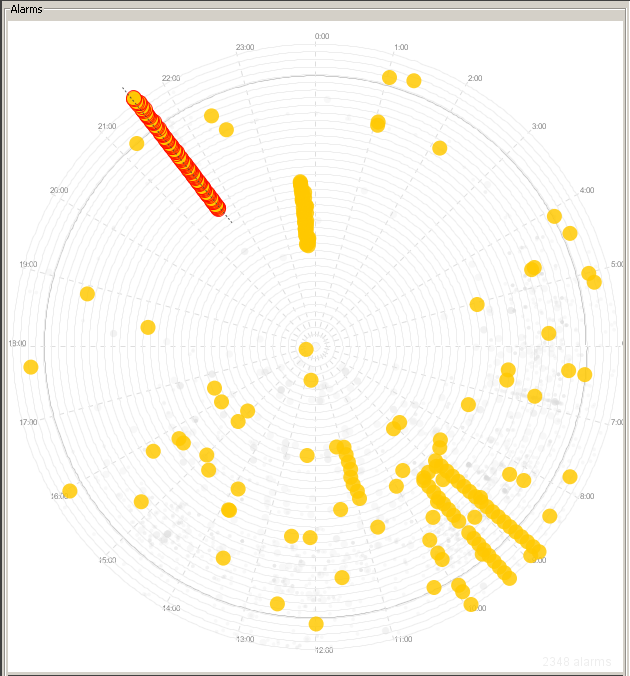
\includegraphics[scale=0.5]{spiral.png}
\vskip 0.5cm}}
\caption{\protect\label{spiral}Spiralview showing IDS logs over time. \cite{bertini2007spiralview}}
\end{figure}

Integrated visualisation system \cite{mukosaka2007integrated} is an IDS log based visualisation tool, focusing on attacks originating inside the monitored network, as these events are less well studied and have important security implications for the network. The tool provides a unified logical, geographic and temporal display of data, using three orthogonal planes. Multiple layouts of the three planes are available, with animated transitions. 

\begin{figure}[tbh]
\fbox{\parbox[b]{.99\linewidth}{
\vskip 0.5cm
\centering 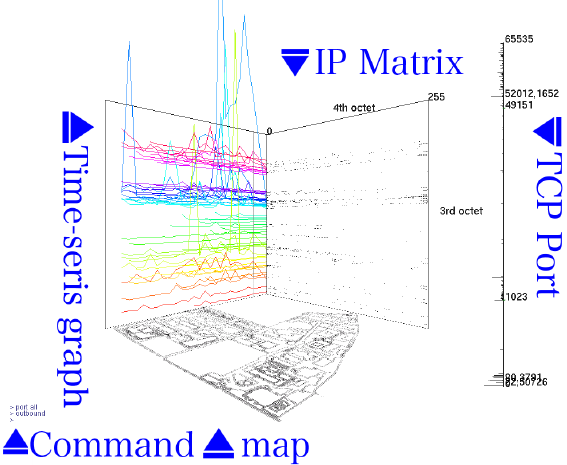
\includegraphics[scale=1]{integrated.png}
\vskip 0.5cm}}
\caption{\protect\label{integrated}Overview of integrated IDS visualisation system \cite{mukosaka2007integrated}. Newer events appear to the right of the time plane.}
\end{figure}

When in the configuration shown in Figure \ref{integrated}, the timeline plane shows events for the entire subnet x.y.x.*. Individual IP's can be chosen by shifting the timeline plane along the IP plane.
Filtering tools are made available to control what kinds of events are shown, though are not described in any kind of detail. port at least is usable to filter on. 

This system relies colour to distinguish ports on the timeline frame, which is easily subject to visual overload, as the human eye is not able to reliably distinguish fine differences in colours. Vertical position of the line indicates the number of events. With poorly described filtering systems and reliance on colour coding to distinguish ports, this system is extremely vulnerable to producing data overload. This leads to missing of important events. the lack of data hiding creates visual clutter which can easily mask important intrusions composed of a small number of events. 

This system appears interesting as an attempt to correlate attack information with machine location through geoip systems. Where the number of events is "low enough" lines are drawn from IP plane to physical location on the lower plane. The exact number of lines drawn is not clear. 

\section{Requirements}\label{reqs}

In order to meet the goals laid out in Chapter \ref{C:intro} concrete requirements have been laid out for the tool.
These requirements are divided into functional and non-functional requirements. Requirements 1 through 3 and 6 support goals 1 and 2. Requirements 3 through 7 support goal 3. Scaling goals are supported by all requirements, as goals 1 and 2 strongly support scaling to millions of events.  

\begin{enumerate}
\item{Strong filtering and highlighting options.}
\item{Show surrounding context for anomalous accesses.}
\item{GeoIP support to add context to login attempts.}
\item{Allow the user control over which machine is monitored at any given time.}
\item{Show network context for currently monitored machine.}
\item{Extensible log parsing: don't prevent extension to other similar log types.}
\end{enumerate}

Non functional requirements deal with issues of performance, scalability and usability.
\begin{enumerate}
\item{Use information hiding to prevent information overload.}
\item{Prevent masking of important data.}
\item{Navigation: tool needs to support easy navigation of the timeline.}
\item{Performance capable of handling millions of events.}
\end{enumerate}